% !TeX program = pdflatex
% !TeX encoding = UTF-8
\documentclass[12pt,a4paper]{article}

\usepackage[utf8]{inputenc}
\usepackage[T1]{fontenc}
\usepackage{lmodern}
\usepackage[brazil]{babel}
\usepackage{listings}
\usepackage{xcolor}
\usepackage{graphicx}
\usepackage{float}
\usepackage{geometry}
\usepackage{indentfirst}
\usepackage{titlesec}
\usepackage{amsmath}
\usepackage{booktabs}
\usepackage{longtable}
\usepackage{tikz}
\usetikzlibrary{arrows.meta,positioning,fit}
\usepackage[hidelinks,pdftitle={Tarefa 18: Comparando Soma de Vetores entre CPU e GPU em OpenMP},pdfauthor={Matheus Bezeril Pinto}]{hyperref}

\geometry{a4paper,top=3cm,bottom=2cm,left=3cm,right=2cm}
\setlength{\parindent}{1.25cm}
\setlength{\parskip}{0.2cm}
\setlength{\emergencystretch}{2em}
\titleformat{\section}{\bfseries\large}{\thesection}{1em}{}
\titleformat{\subsection}{\bfseries\normalsize}{\thesubsection}{1em}{}
\graphicspath{{figuras/}}
\renewcommand{\lstlistingname}{Código}
\renewcommand{\lstlistlistingname}{Lista de códigos}
\definecolor{shellFont}{RGB}{233,233,233}
\definecolor{shellBG}{RGB}{44,51,122}
\definecolor{shellKeywords}{RGB}{250,227,0}
\definecolor{shellString}{RGB}{250,166,0}

\lstdefinestyle{Base}{
    basicstyle=\ttfamily\footnotesize,
    numbers=left,numberstyle=\tiny,numbersep=8pt,
    tabsize=4,breaklines=true,breakatwhitespace=false,
    showstringspaces=false,frame=single,
    columns=fullflexible,keepspaces=true,
    inputencoding=utf8,extendedchars=true,
    literate=
    {á}{{\'a}}1 {à}{{\`a}}1 {ã}{{\~a}}1 {â}{{\^a}}1
    {é}{{\'e}}1 {ê}{{\^e}}1 {í}{{\'i}}1
    {ó}{{\'o}}1 {ô}{{\^o}}1 {õ}{{\~o}}1
    {ú}{{\'u}}1 {ç}{{\c{c}}}1
    {Á}{{\'A}}1 {À}{{\`A}}1 {Ã}{{\~A}}1 {Â}{{\^A}}1
    {É}{{\'E}}1 {Ê}{{\^E}}1 {Í}{{\'I}}1
    {Ó}{{\'O}}1 {Ô}{{\^O}}1 {Õ}{{\~O}}1
    {Ú}{{\'U}}1 {Ç}{{\c{C}}}1
    {−}{{\ensuremath{-}}}1 {×}{{\ensuremath{\times}}}1
    {²}{{\ensuremath{^2}}}1
}
\lstdefinestyle{CStyle}{
    style=Base,language=C,
    keywordstyle=\color{blue}\bfseries,
    stringstyle=\color{red},
    commentstyle=\color{green!50!black},
    backgroundcolor=\color{gray!10}
}
\lstdefinestyle{Terminal}{
    style=Base,language=bash,
    basicstyle=\ttfamily\footnotesize\color{shellFont},
    keywordstyle=\color{shellKeywords}\bfseries,
    stringstyle=\color{shellString},
    commentstyle=\color{gray!30},
    numberstyle=\tiny\color{black},
    backgroundcolor=\color{shellBG}
}


\lstdefinestyle{Apendice}{
    style=CStyle,
    basicstyle=\fontsize{8.5}{10}\selectfont\ttfamily,
    numberstyle=\tiny,numbersep=7pt,
    backgroundcolor=\color{gray!4},
    xleftmargin=1em,framexleftmargin=.3em
}
\lstdefinestyle{Dados}{
    style=Apendice,language={},
    keywordstyle={},commentstyle={},stringstyle={},
    numbers=none,backgroundcolor=\color{white}
}

\title{\textbf{Tarefa 18: Comparando Soma de Vetores entre CPU e GPU em OpenMP}}
\author{Matheus Bezeril Pinto}
\date{Outubro de 2026}

\begin{document}
\maketitle

\section*{Resumo}
Este relatório compara a soma de vetores em CPU e em GPU NVIDIA Tesla V100 com OpenMP. Foram analisadas três séries CPU e três séries V100, totalizando 30 medições e três execuções de aquecimento. Cada execução soma dez milhões de elementos em precisão simples. As médias CPU foram de $10{,}568$ ms e $9{,}975$ ms com uma thread configurada, e $5{,}379$ ms com quatro. Na V100, as médias ficaram entre $12{,}176$ ms e $13{,}484$ ms. Todos os registros apresentaram zero erros. A CPU foi mais rápida na operação medida. A interpretação considera a baixa quantidade de cálculo por elemento e os custos de movimentar os dados e iniciar a execução na GPU. Como os logs medem a chamada completa, não se atribui uma parcela numérica do tempo às transferências ou ao kernel isoladamente. O texto explica as diretivas, o intervalo medido e a dispersão dos tempos; os códigos e os registros completos estão nos apêndices.

\section{Objetivo e seleção das execuções}
O enunciado solicita realizar os exercícios de adição de vetores do tutorial de GPUs com OpenMP no NPAD, comparar CPU e GPU e apresentar os problemas encontrados e as soluções adotadas \cite{enunciado,tutorial}. A comparação deve considerar o que está dentro da medição: executar uma operação completa com dados inicialmente no host pode ter um resultado diferente de medir apenas um kernel com dados já na GPU.

A implementação está organizada nos arquivos \texttt{t18.c}, \texttt{aux18.c}, \texttt{somas.c} e \texttt{jobs.sh} \cite{repositorio}. A análise utiliza as três séries CPU e as três séries com Tesla V100-SXM2-16GB. Foram mantidos o mesmo tamanho dos vetores e a mesma tolerância; as execuções com outros aceleradores não integram a comparação. A identificação dos registros é:

\begin{table}[H]
\centering\small
\begin{tabular}{lp{8cm}l}
\toprule
Série & Arquivo original & Configuração\\
\midrule
CPU 1a & \texttt{CPU1a.out} & CPU, 1 thread\\
CPU 1b & \texttt{CPU1b.out} & CPU, 1 thread\\
CPU 4 & \texttt{CPU4.out} & CPU, 4 threads\\
V100 a & \texttt{GPUa.out} & GPU V100\\
V100 b & \texttt{GPUb.out} & GPU V100\\
V100 c & \texttt{resultado\_gpu\_2134904.out} & GPU V100\\
\bottomrule
\end{tabular}
\caption{Arquivos utilizados na comparação CPU/V100. As estatísticas são calculadas separadamente para cada série.}
\label{tab:selecao}
\end{table}

O enunciado cita os slides 27 e 48. Na edição SC23 disponível no tutorial NPAD consultado, os exercícios equivalentes aparecem nas páginas 29 e 50 do PDF: primeiro a distribuição do laço na CPU, depois o uso de \texttt{target} e \texttt{loop} na GPU.

\section{Operação e quantidade de trabalho}
\subsection{Soma elemento a elemento}
Dados os vetores $a$ e $b$, calcula-se
\[
c_i=a_i+b_i,\qquad i=0,\ldots,N-1.
\]
Cada resultado depende apenas de duas entradas com o mesmo índice. Não existe uma soma acumulada entre posições. Por isso, diferentes índices podem ser processados simultaneamente, sem que uma iteração precise esperar pelo resultado de outra.

\begin{figure}[H]
\centering
\begin{tikzpicture}[font=\small,>=Latex,
  celula/.style={draw=blue!60!black,fill=blue!5,minimum width=1.75cm,minimum height=.65cm}]
\foreach \i [count=\k from 0] in {0,1,2,3}{
  \node[celula] (a\k) at (\k*2.45,2.2) {$a[\i]$};
  \node[celula] (b\k) at (\k*2.45,1.1) {$b[\i]$};
  \node[celula,fill=orange!15,draw=orange!70!black] (c\k) at (\k*2.45,-.4) {$c[\i]$};
  \node (s\k) at (\k*2.45,.35) {$+$};
  \draw[->] (b\k)--(s\k);
  \draw[->] (s\k)--(c\k);
  \draw[->] (a\k.east) -- ++(.28,0) |- (s\k.east);
}
\node[anchor=west] at (8.65,1.1) {$\cdots$};
\node[align=center,text width=12cm] at (3.7,-1.3)
{Cada índice pode ser calculado independentemente.\\Não há soma acumulada entre posições.};
\end{tikzpicture}
\caption{Adição elemento a elemento. A independência entre índices permite distribuir o laço na CPU ou em um dispositivo com offload.}
\label{fig:vetores}
\end{figure}


Nesta implementação, $N=10^7$, os vetores usam \texttt{float}, $a_i$ recebe a conversão de $i$, $b_i$ recebe duas vezes esse valor e $c_i$ começa zerado. O vetor \texttt{res} guarda a expressão de referência $a_i+b_i$, também em precisão simples, para a comparação final.

\subsection{Intensidade aritmética e volume de dados}
Com quatro bytes por \texttt{float}, cada vetor ocupa 40 MB. Os quatro vetores no host ocupam 160 MB: duas entradas, uma saída e uma referência. Os dados úteis da soma são 80 MB de entrada e 40 MB de saída.

Cada elemento exige uma adição, duas leituras e uma escrita. A \textit{intensidade aritmética}, isto é, a quantidade de cálculo em relação aos dados acessados, é aproximadamente
\[
I=\frac{1\text{ operação}}{12\text{ bytes}}
\approx0{,}083\text{ operação/byte}.
\]
Essa relação é pequena: o algoritmo movimenta dados para realizar apenas uma soma por elemento. Portanto, uma grande capacidade de cálculo da GPU não garante uma chamada mais rápida quando é necessário disponibilizar as entradas no dispositivo e devolver o resultado ao host.

\begin{figure}[H]
\centering
\begin{tikzpicture}[font=\small,>=Latex,
  caixa/.style={draw=blue!65!black,fill=blue!5,text width=3.5cm,minimum height=2.35cm,align=center}]
\node[caixa] (h) at (0,0) {\textbf{Host / CPU}\\[4pt]Vetores em \texttt{malloc}\\$a$, $b$, $c$ e referência};
\node[caixa,fill=orange!12,draw=orange!70!black] (d) at (8,0)
{\textbf{Dispositivo / GPU}\\[4pt]Dados acessíveis no dispositivo\\$c[i]=a[i]+b[i]$};
\draw[->,thick] (h.30)--node[above,align=center,font=\footnotesize]
{Entradas: $a$ e $b$\\80 MB de dados} (d.150);
\draw[->,thick] (d.210)--node[below,align=center,font=\footnotesize]
{Saída: $c$\\40 MB de dados} (h.330);
\node[align=center,text width=12.3cm] at (4,-2.65)
{Cada vetor possui dez milhões de elementos.\\A referência fica no host para a validação.};
\end{tikzpicture}
\caption{Modelo de movimentação dos dados úteis entre host e dispositivo. O desenho representa as entradas e a saída necessárias à operação, sem medir o tráfego efetivo do runtime.}
\label{fig:offload}
\end{figure}


A figura representa as regiões de dados úteis de uma transferência explícita. Não é uma medição de tráfego. A implementação utiliza ponteiros de \texttt{malloc} sem cláusulas \texttt{map} explícitas; a forma efetiva de disponibilizar esses dados depende do suporte e do modelo de memória do compilador e do runtime. Os logs não registram bytes transferidos, e os 120 MB não são apresentados como uma medição dessas transferências.

\section{Implementação e conceitos de OpenMP}
\subsection{Organização dos arquivos}
\texttt{t18.c} recebe tamanho, tolerância e modo, chama as etapas e mede a soma. \texttt{aux18.c} contém leitura dos argumentos, alocação, inicialização, validação e liberação. \texttt{somas.c} contém as duas funções de soma. \texttt{jobs.sh} solicita recursos ao Slurm, compila e executa as repetições.

Os dois arquivos auxiliares são incluídos diretamente em \texttt{t18.c}. Portanto, o comando compila somente \texttt{t18.c}; adicionar os mesmos arquivos novamente ao comando produziria definições duplicadas. A alocação com \texttt{malloc} permite reservar os vetores no heap, evitando depender de espaço suficiente na pilha para quatro arrays grandes. As conversões dos argumentos verificam formato e faixa, e as alocações são verificadas antes do uso.

\subsection{CPU: distribuição do laço com parallel for}
\begin{lstlisting}[style=CStyle]
#pragma omp parallel for
for (int i = 0; i < N; i++) {
    c[i] = a[i] + b[i];
}
\end{lstlisting}
A diretiva cria uma região paralela e distribui as iterações pela equipe de threads. Cada thread escreve em elementos diferentes de $c$. A sincronização ao final garante que a soma esteja concluída antes da continuação do programa.

O percurso em índices crescentes acessa posições contíguas dos vetores. Isso favorece a localidade espacial: uma linha de cache traz dados próximos que poderão ser usados nas próximas iterações. O compilador também pode vetorizar a soma, processando vários elementos por instrução. Vetorização e distribuição entre threads são mecanismos distintos.

\subsection{GPU: target, loop e MANDATORY}
\begin{lstlisting}[style=CStyle]
#pragma omp target
#pragma omp loop
for (int i = 0; i < N; i++) {
    c[i] = a[i] + b[i];
}
\end{lstlisting}
\texttt{target} delimita a região destinada ao dispositivo; \texttt{loop} descreve o laço que pode ser distribuído no contexto de execução disponível. O encaminhamento da execução do host para o dispositivo é chamado \textit{offload}. Nesta tarefa, o host inicia o programa e realiza a validação, enquanto o modo GPU utiliza a região target para a soma \cite{openmp}.

O job GPU contém explicitamente:
\begin{lstlisting}[style=Terminal]
export OMP_TARGET_OFFLOAD=MANDATORY
\end{lstlisting}
No padrão OpenMP, \texttt{MANDATORY} exige a execução no dispositivo para essas regiões target e determina falha caso o offload não possa ser realizado, em vez de permitir uma execução silenciosa no host, chamada \textit{fallback}. Essa política foi definida no job das execuções V100. Seu funcionamento pressupõe compilador e runtime compatíveis com offload e com as diretivas utilizadas.

A variável define a política de execução. Ela não divide automaticamente o vetor entre GPUs, não especifica o mapeamento dos vetores e não mantém os dados disponíveis entre processos distintos. Assim, exigir o uso da GPU não elimina os custos que entram na chamada medida.

\subsection{Validação e redução}
Depois da soma, o programa conta as posições em que
\[
|c_i-\mathrm{res}_i|>10^{-9}.
\]
A contagem usa \texttt{parallel for reduction(+:err)}: cada thread acumula sua contribuição, e as contribuições são somadas ao final. Isso evita atualizações concorrentes desprotegidas no mesmo contador.

Todos os 33 registros selecionados, incluindo os aquecimentos, mostraram zero erros pelo critério implementado. A referência usa a mesma expressão em \texttt{float}; esse resultado verifica a soma nesse critério, sem significar precisão decimal de nove casas. A validação fica fora do intervalo cronometrado.

\section{Ambiente e metodologia}
\subsection{Recursos do NPAD}
Os logs CPU identificam \texttt{service3.npad.internal}, com uma ou quatro threads configuradas. Os logs V100 identificam \texttt{gpunode1.npad.internal} e Tesla V100-SXM2-16GB. A documentação de hardware do NPAD informa que a classe \texttt{gpu-8-v100} possui, por nó, dois Intel Xeon E5-2683 v4, 512 GB DDR4 e oito GPUs V100 com 16 GB por GPU \cite{hardware}. RAM do host e memória da GPU são recursos distintos. O modelo da CPU de \texttt{service3} não consta dos registros do experimento.

O script CPU solicita \texttt{intel-128}, um nó e uma tarefa. O script apresentado configura uma CPU por tarefa; o log CPU 4 documenta a variação com quatro threads. A quantidade configurada é exportada para \path{OMP_NUM_THREADS}. As variáveis \path{OMP_PLACES=cores} e \path{OMP_PROC_BIND=close} orientam o posicionamento das threads nos locais de execução.

O script GPU solicita a partição \texttt{gpu-8-v100} e quatro GPUs. A quantidade de GPUs existentes no nó ou reservadas ao job não equivale à quantidade usada pelo algoritmo: o fonte possui uma região target e não implementa uma divisão do vetor entre dispositivos.

\begin{figure}[H]
\centering
\begin{tikzpicture}[font=\small,>=Latex,
  gpu/.style={draw=gray!65,fill=gray!5,text width=2.05cm,minimum height=.85cm,align=center}]
\node[draw=blue!65!black,fill=blue!5,rounded corners,align=center,
      text width=3.6cm,minimum height=1.1cm] (p) at (0,0)
{Um processo\\Uma região \texttt{target}};
\node[gpu,draw=orange!75!black,fill=orange!18] (a) at (5.7,1.5) {Dispositivo padrão};
\node[gpu] (b) at (9.2,1.5) {Outro dispositivo};
\node[gpu] (c) at (5.7,-.3) {Outro dispositivo};
\node[gpu] (d) at (9.2,-.3) {Outro dispositivo};
\draw[->,thick] (p.east) -- ++(.6,0) |- (a.west);
\node[draw=gray!60,dashed,fit=(a)(b)(c)(d),inner sep=8pt,
      label={[font=\footnotesize]below:Exemplo: quatro GPUs visíveis na alocação}] {};
\end{tikzpicture}
\caption{Oito GPUs no nó e quatro GPUs solicitadas ao Slurm não significam uma soma distribuída por quatro dispositivos. O programa possui uma região target, sem particionamento explícito do vetor entre GPUs.}
\label{fig:dispositivos}
\end{figure}


Os dois modos utilizam o comando de compilação apresentado no job, com \texttt{-O3}, OpenMP e C11:
\begin{lstlisting}[style=Terminal]
gcc -O3 -fopenmp -std=c11 t18.c -o executavel -lm
\end{lstlisting}
O nome do executável e o argumento final selecionam CPU ou GPU. As comparações preservam $N=10^7$ e tolerância $10^{-9}$; não se misturam resultados de outras classes de aceleradores.

\subsection{Intervalo de medição}
\texttt{omp\_get\_wtime()} é chamado antes e depois de \texttt{soma\_cpu} ou \texttt{soma\_gpu}. O número impresso é o tempo da chamada completa. Alocação, inicialização, construção da referência, verificação e impressão ficam fora desse intervalo.

\begin{figure}[H]
\centering
\begin{tikzpicture}[font=\small,>=Latex,
  fase/.style={draw=gray!70,fill=gray!7,text width=3.25cm,minimum height=1.3cm,align=center}]
\node[fase] (a) at (0,0) {Alocar e inicializar\\$a$, $b$, $c$ e referência};
\node[fase,fill=orange!18,draw=orange!75!black] (b) at (4.45,0)
{\texttt{soma\_cpu}\\ou \texttt{soma\_gpu}};
\node[fase] (c) at (8.9,0) {Verificar, imprimir\\e liberar memória};
\draw[->,thick] (a)--(b);
\draw[->,thick] (b)--(c);
\node[font=\footnotesize,above=3pt of b] {Intervalo cronometrado};
\draw[orange!80!black,thick] (2.62,-.85)--(6.28,-.85);
\node[align=center,text width=12.3cm] at (4.45,-1.7)
{Em offload com transferência explícita, a chamada inclui envio,\\execução e retorno dos dados. Os logs não separam esses custos.};
\end{tikzpicture}
\caption{O tempo impresso mede a chamada completa de soma. Não inclui inicialização nem validação; a região target é síncrona no código apresentado.}
\label{fig:tempo}
\end{figure}


A região target não usa \texttt{nowait}; a chamada espera sua conclusão. Assim, o tempo GPU é avaliado como o custo da operação a partir dos dados no host, incluindo os custos de offload presentes no caminho executado. Não se trata de uma medição isolada do kernel com os dados previamente residentes na GPU.

\subsection{Repetições, aquecimento e CV}
São seis séries de cinco medições: 30 tempos utilizados nas médias. As três séries V100 possuem uma execução anterior identificada como \texttt{Warm-up}, excluída da média, totalizando 33 registros preservados.

Cada chamada ao executável inicia um processo e realiza uma soma. Por isso, o aquecimento anterior não garante reutilizar o mesmo contexto de GPU no processo seguinte. As cinco medições continuam sujeitas aos custos iniciais presentes em cada chamada. Isso caracteriza o experimento, em vez de uma avaliação de um contexto persistente já aquecido.

Para cinco tempos $T_r$, usam-se média $\overline T$, desvio padrão amostral $s$ e coeficiente de variação:
\[
\overline T=\frac{1}{5}\sum_{r=1}^{5}T_r,\qquad
s=\sqrt{\frac{\sum_{r=1}^{5}(T_r-\overline T)^2}{4}},\qquad
CV=100\frac{s}{\overline T}.
\]
O \textit{coeficiente de variação} (CV) expressa a dispersão dos tempos em relação à média. Por exemplo, média de 10 ms e desvio de 0,2 ms correspondem a CV de $2\%$. Um CV baixo indica tempos próximos entre si; não significa menor tempo, menor erro numérico ou maior eficiência da GPU. As barras do gráfico representam um desvio padrão amostral.

\section{Resultados CPU e V100}
\subsection{Tempos médios e dispersão}
{\small\begin{longtable}{lrrrr}
\caption{Séries CPU e Tesla V100. Cinco medições por série; aquecimentos separados e excluídos das médias.}\label{tab:resumo}\\
\toprule Série & Média (ms) & $s$ (ms) & CV (\%) & Aquecimento (ms)\\
\midrule\endfirsthead
\toprule Série & Média (ms) & $s$ (ms) & CV (\%) & Aquecimento (ms)\\
\midrule\endhead
\bottomrule\endfoot
CPU 1a & 10,567663 & 0,019582 & 0,19 & ---\\
CPU 1b & 9,974812 & 0,038587 & 0,39 & ---\\
CPU 4 & 5,379129 & 0,037736 & 0,70 & ---\\
V100 a & 12,927817 & 0,127933 & 0,99 & 13,064327\\
V100 b & 13,484205 & 0,339940 & 2,52 & 14,371583\\
V100 c & 12,175676 & 0,339729 & 2,79 & 12,091021\\
\end{longtable}
}

\begin{figure}[H]
\centering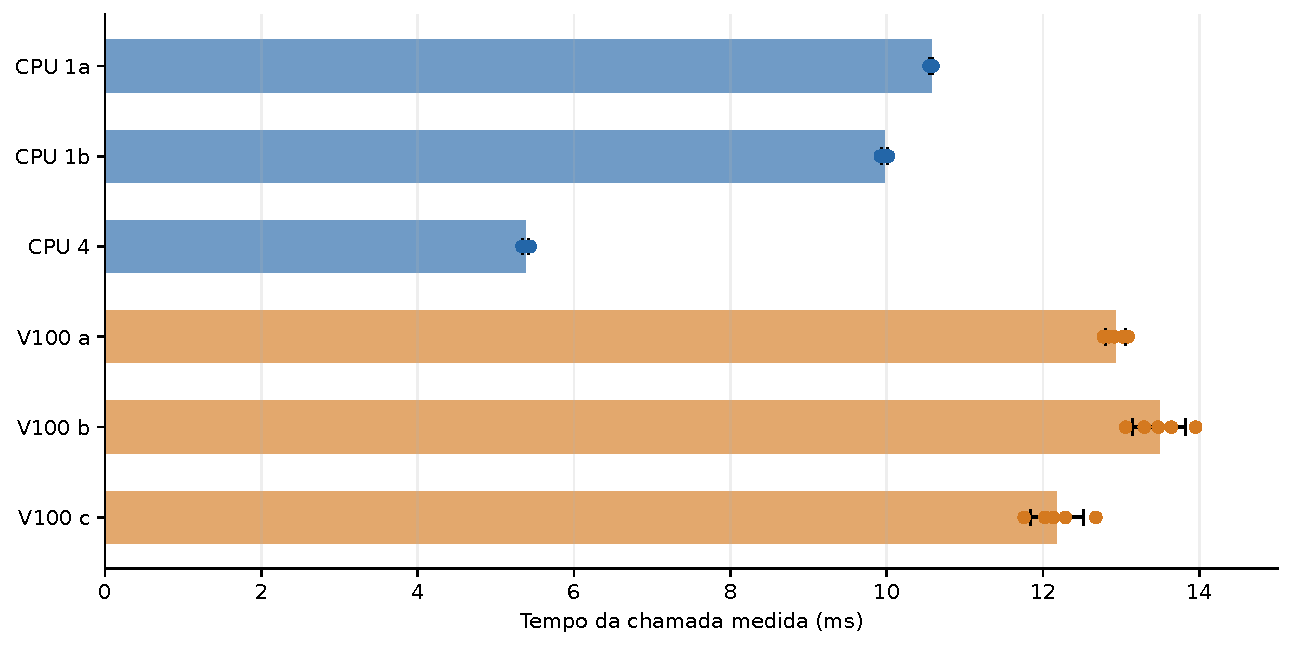
\includegraphics[width=\linewidth]{tempos.pdf}
\caption{As 30 medições selecionadas, com médias e desvios amostrais. Azul: CPU. Laranja: V100. Os três aquecimentos GPU não entram no gráfico nem nas médias.}
\label{fig:tempos}
\end{figure}

A CPU com quatro threads apresentou a menor média, $5{,}379$ ms. As duas séries CPU de uma thread também foram mais rápidas que todas as séries V100. Os CVs variam de aproximadamente $0{,}19\%$ a $2{,}79\%$, indicando pequena dispersão interna nas séries.

As médias CPU 1a e CPU 1b diferem cerca de $5{,}94\%$, mais que seus desvios internos. Portanto, as duas referências são mantidas separadas. O mesmo cuidado é aplicado às três séries V100: não se escolhe apenas a mais rápida para representar todo o experimento.

\subsection{Ganho com quatro threads na CPU}
O speedup relativo e a eficiência com quatro threads são
\[
S_4=\frac{\overline T_1}{\overline T_4},\qquad E_4=\frac{S_4}{4}.
\]
{\small\begin{longtable}{lrrr}
\caption{Comparação CPU com o mesmo N. As duas referências permanecem separadas.}\label{tab:cpu}\\
\toprule Referência de uma thread & $T_1/T_4$ & $E_4$ (\%) & $T_4$ (ms)\\
\midrule\endfirsthead
\toprule Referência de uma thread & $T_1/T_4$ & $E_4$ (\%) & $T_4$ (ms)\\
\midrule\endhead
\bottomrule\endfoot
CPU 1a & 1,9646 & 49,11 & 5,379129\\
CPU 1b & 1,8544 & 46,36 & 5,379129\\
\end{longtable}
}

A aceleração fica entre $1{,}854$ e $1{,}965$, conforme a referência de uma thread, e a eficiência entre $46{,}36\%$ e $49{,}11\%$. Isso corresponde a um ganho próximo de duas vezes ao usar quatro threads. Eficiência aqui é a aproximação ao ganho ideal de quatro vezes, não a porcentagem de utilização da CPU.

O acesso contíguo favorece caches e vetorização, mas várias threads compartilham recursos de memória e precisam ser coordenadas. Como há pouco cálculo por elemento, o ganho não precisa acompanhar proporcionalmente o número de threads. Os logs não separam os custos desses mecanismos.

\subsection{Comparação da chamada GPU com a CPU}
{\small\begin{longtable}{lrrr}
\caption{Razão entre tempos médios. Valores maiores que um indicam maior tempo da chamada GPU em relação à referência CPU da coluna.}\label{tab:comparacao}\\
\toprule Série & $T_{GPU}/T_{CPU\,1a}$ & $T_{GPU}/T_{CPU\,1b}$ & $T_{GPU}/T_{CPU\,4}$\\
\midrule\endfirsthead
\toprule Série & $T_{GPU}/T_{CPU\,1a}$ & $T_{GPU}/T_{CPU\,1b}$ & $T_{GPU}/T_{CPU\,4}$\\
\midrule\endhead
\bottomrule\endfoot
V100 a & 1,223 & 1,296 & 2,403\\
V100 b & 1,276 & 1,352 & 2,507\\
V100 c & 1,152 & 1,221 & 2,264\\
\end{longtable}
}

As médias V100 ficaram entre $12{,}176$ ms e $13{,}484$ ms. Em relação à CPU com quatro threads, a chamada GPU demorou aproximadamente $2{,}26$ a $2{,}51$ vezes mais. A vantagem CPU também aparece nas duas referências de uma thread, embora seja menor.

Essa comparação responde à operação medida: somar os vetores a partir da organização de dados do programa. Ela não demonstra que uma soma com os dados já disponíveis na V100 seria mais lenta que o laço CPU, pois esse cenário não foi medido separadamente.

\section{Discussão dos custos de execução}
\subsection{Tempo total e tempo do kernel}
O \textit{kernel} é a parte do cálculo executada no dispositivo. Para uma operação com dados inicialmente no host e transferência explícita, um modelo conceitual do tempo é
\[
T_{GPU}=T_{\text{envio}}+T_{\text{preparação}}+T_{\text{kernel}}+T_{\text{retorno}}+T_{\text{sincronização}}.
\]
Na CPU, os vetores já estão na memória do host. Também existe custo para lê-los e escrever a saída, mas não é necessário disponibilizá-los em outro dispositivo e trazer o resultado de volta. Uma GPU pode executar o kernel rapidamente e, ainda assim, perder na soma desses custos.

\begin{figure}[H]
\centering
\begin{tikzpicture}[font=\small,>=Latex,
  fase/.style={draw=blue!65!black,fill=blue!5,text width=2.55cm,
               minimum height=1.2cm,align=center}]
\node[anchor=east] at (-1.8,1.8) {CPU};
\node[draw=blue!65!black,fill=blue!5,align=center,
      text width=11.2cm,minimum height=1cm] at (4,1.8)
{Ler as entradas, somar e escrever o resultado na memória do host};
\node[anchor=east] at (-1.8,0) {GPU};
\node[fase] (a) at (0,0) {Enviar $a$ e $b$\\80 MB};
\node[fase,fill=gray!10,draw=gray!65] (b) at (3.5,0)
{Preparar e lançar\\o cálculo};
\node[fase,fill=orange!18,draw=orange!75!black] (c) at (7,0)
{Somar\\$c_i=a_i+b_i$};
\node[fase] (d) at (10.5,0) {Trazer $c$\\40 MB};
\draw[->,thick] (a)--(b);
\draw[->,thick] (b)--(c);
\draw[->,thick] (c)--(d);
\node[align=center,text width=14cm] at (4.7,-1.5)
{O tempo total da chamada depende de todas as etapas.\\Uma soma por elemento oferece pouco cálculo para amortizar a movimentação.};
\end{tikzpicture}
\caption{Custos de uma soma com dados inicialmente no host e transferência explícita. Os blocos não estão em escala de tempo e não representam uma decomposição medida. O envio e o retorno ocorrem na entrada e na saída da região, não uma vez por iteração do laço.}
\label{fig:custos}
\end{figure}


A interpretação adotada para o resultado é que a movimentação dos dados e os custos de offload não foram compensados pelo pouco cálculo realizado. Cada elemento participa de apenas uma soma. O potencial de paralelismo da GPU não elimina o tempo necessário para disponibilizar as entradas, iniciar a execução e retornar a saída.

A movimentação considerada ocorre por regiões dos vetores, sem pressupor uma cópia a cada iteração de \texttt{for}. Para a soma completa, são duas regiões de entrada e uma de saída, representadas pelos 120 MB de dados úteis. Em cada novo processo, o programa realiza novamente sua operação, sem reutilizar dados de uma chamada anterior. O custo é grande em relação ao trabalho matemático, mesmo sem uma cópia por elemento.

\subsection{Alcance da análise}
Os tempos mostram a vantagem CPU para essa soma e essa forma de medição. A comparação envolve nós distintos e se restringe às configurações testadas. A baixa intensidade aritmética oferece uma explicação coerente para o peso da movimentação. Entretanto, os logs não medem envio, kernel e retorno separadamente. Portanto, não se atribui uma porcentagem específica às transferências nem se calcula uma largura de banda a partir de um tempo que inclui outras etapas.

Um algoritmo que realize mais operações por elemento ou aproveite os dados em vários cálculos oferece mais trabalho para amortizar a movimentação. Apenas aumentar $N$ mantém a mesma proporção de uma soma por elemento, embora possa reduzir a importância relativa de custos fixos de lançamento.

\section{Progresso e decisões de implementação}
\begin{table}[H]
\centering\small
\begin{tabular}{p{3cm}p{5.1cm}p{5.1cm}}
\toprule
Questão & Decisão adotada & Motivo\\
\midrule
Vetores grandes & Alocação com \texttt{malloc} e teste de falha & Reservar memória sem depender de grandes arrays na pilha.\\[3pt]
Entradas inválidas & Conversão com checagem de formato e faixa & Evitar tamanhos, tolerâncias e modos inválidos.\\[3pt]
Laço CPU & \texttt{parallel for} & Distribuir índices independentes entre threads.\\[3pt]
Modo GPU & \texttt{target}, \texttt{loop} e política \texttt{MANDATORY} no job & Destinar o cálculo ao dispositivo e exigir offload na configuração OpenMP.\\[3pt]
Verificação & Referência e \texttt{reduction(+:err)} & Comparar a saída e combinar as contagens sem disputa no contador.\\[3pt]
Comparação de tempos & Mesmos vetores e intervalo em torno da soma & Comparar a operação completa, explicitando seus custos.\\
\bottomrule
\end{tabular}
\caption{Principais decisões da implementação e suas finalidades.}
\end{table}

\section{Conclusão}
Na soma de dez milhões de elementos, a CPU apresentou menor tempo que a V100 em todas as séries selecionadas. Com quatro threads, a média CPU foi de $5{,}379$ ms; na V100, ficou entre $12{,}176$ ms e $13{,}484$ ms. Todos os registros apresentaram zero erros pelo verificador implementado.

O resultado é interpretado a partir do custo da operação completa e da baixa intensidade aritmética: movimentar os dados e iniciar a execução na GPU não foi compensado por apenas uma soma por elemento. A configuração \texttt{MANDATORY} define a exigência de offload, mas não elimina esses custos. A medição não separa as parcelas para quantificá-las individualmente.

Os resultados mostram que a escolha do recurso de execução depende da quantidade de cálculo por dado e do intervalo efetivamente medido. Para este trabalho simples, a CPU foi a opção mais rápida; a capacidade de cálculo da GPU, sozinha, não determina o desempenho da aplicação completa.

\clearpage\appendix
\section{Enunciado e proveniência}
\subsection{Requisitos completos}
\lstinputlisting[style=Dados]{dados/requisitosTarefa18.txt}
\subsection{Seleção e proveniência dos arquivos}
\lstinputlisting[style=Dados]{dados/proveniencia.txt}
\subsection{Referência de hardware da classe V100}
\lstinputlisting[style=Dados]{dados/hardware_referencia.txt}

\clearpage\section{Códigos completos}
Os códigos e o script utilizados são apresentados integralmente a seguir. A inclusão usa \texttt{\textbackslash lstinputlisting}, sem limites de linhas, para manter os apêndices sincronizados com os arquivos do projeto.
\subsection{Programa principal: t18.c}
\lstinputlisting[style=Apendice]{codigos/t18.c}
\clearpage\subsection{Somas CPU e GPU: somas.c}
\lstinputlisting[style=Apendice]{codigos/somas.c}
\subsection{Funções auxiliares: aux18.c}
\lstinputlisting[style=Apendice]{codigos/aux18.c}
\clearpage\subsection{Submissão: jobs.sh}
\lstinputlisting[style=Apendice,language=bash]{codigos/jobs.sh}

\clearpage\section{Medições completas e identificação dos arquivos}
Os aquecimentos são as repetições zero. Todos os valores pertencem às séries CPU e V100 selecionadas; as médias utilizam somente as cinco repetições medidas de cada série.
{\small\begin{longtable}{lrrr}
\caption{Todos os 39 registros. Repetição 0 identifica o aquecimento em processo separado.}\label{tab:brutos}\\
\toprule Série & Repetição & Tempo (s) & Erros\\
\midrule\endfirsthead
\toprule Série & Repetição & Tempo (s) & Erros\\
\midrule\endhead
\bottomrule\endfoot
CPU 1a & 1 & 0,010591173 & 0\\
CPU 1a & 2 & 0,010564717 & 0\\
CPU 1a & 3 & 0,010541467 & 0\\
CPU 1a & 4 & 0,010558852 & 0\\
CPU 1a & 5 & 0,010582105 & 0\\
CPU 1b & 1 & 0,009982172 & 0\\
CPU 1b & 2 & 0,010022212 & 0\\
CPU 1b & 3 & 0,009961779 & 0\\
CPU 1b & 4 & 0,009917792 & 0\\
CPU 1b & 5 & 0,009990105 & 0\\
CPU 4 & 1 & 0,005374323 & 0\\
CPU 4 & 2 & 0,005372279 & 0\\
CPU 4 & 3 & 0,005439168 & 0\\
CPU 4 & 4 & 0,005334313 & 0\\
CPU 4 & 5 & 0,005375561 & 0\\
V100 a & 0 & 0,013064327 & 0\\
V100 a & 1 & 0,013018875 & 0\\
V100 a & 2 & 0,012913231 & 0\\
V100 a & 3 & 0,013088888 & 0\\
V100 a & 4 & 0,012771590 & 0\\
V100 a & 5 & 0,012846501 & 0\\
V100 b & 0 & 0,014371583 & 0\\
V100 b & 1 & 0,013473431 & 0\\
V100 b & 2 & 0,013641344 & 0\\
V100 b & 3 & 0,013953403 & 0\\
V100 b & 4 & 0,013058480 & 0\\
V100 b & 5 & 0,013294365 & 0\\
H200 & 0 & 0,006105013 & 0\\
H200 & 1 & 0,006026457 & 0\\
H200 & 2 & 0,005933619 & 0\\
H200 & 3 & 0,005993496 & 0\\
H200 & 4 & 0,005984337 & 0\\
H200 & 5 & 0,006045078 & 0\\
V100 / 4 visíveis & 0 & 0,012091021 & 0\\
V100 / 4 visíveis & 1 & 0,012676509 & 0\\
V100 / 4 visíveis & 2 & 0,012025466 & 0\\
V100 / 4 visíveis & 3 & 0,012285496 & 0\\
V100 / 4 visíveis & 4 & 0,011758101 & 0\\
V100 / 4 visíveis & 5 & 0,012132809 & 0\\
\end{longtable}
}
\subsection{Hashes SHA-256 dos fontes e registros selecionados}
\lstinputlisting[style=Dados]{dados/fontes_e_registros.sha256}

\clearpage\section{Registros integrais das execuções selecionadas}
\subsection{CPU1a.out}
\lstinputlisting[style=Dados]{dados/logs/CPU1a.out}
\clearpage\subsection{CPU1b.out}
\lstinputlisting[style=Dados]{dados/logs/CPU1b.out}
\clearpage\subsection{CPU4.out}
\lstinputlisting[style=Dados]{dados/logs/CPU4.out}
\clearpage\subsection{GPUa.out: V100 a}
\lstinputlisting[style=Dados]{dados/logs/GPUa.out}
\clearpage\subsection{GPUb.out: V100 b}
\lstinputlisting[style=Dados]{dados/logs/GPUb.out}
\clearpage\subsection{resultado\_gpu\_2134904.out: V100 c}
\lstinputlisting[style=Dados]{dados/logs/resultado_gpu_2134904.out}

\clearpage\section{Código completo de geração do gráfico e das tabelas}
O script utiliza uma lista explícita de arquivos selecionados e verifica a identificação V100 nos logs GPU. Ele extrai os 33 registros, calcula as estatísticas das 30 medições e gera os artefatos do relatório. Não executa novas simulações.
\lstinputlisting[style=Apendice,language=Python]{gerar_figuras.py}

\clearpage
\begin{thebibliography}{9}
\bibitem{enunciado} Material da disciplina de Programação Paralela. \textit{Tarefa 18: Comparando soma de vetores entre CPU e GPU em OpenMP}. Enunciado reproduzido no Apêndice A.
\bibitem{tutorial} UNIVERSITY OF BRISTOL; NPAD/UFRN. \textit{Programming Your GPU with OpenMP}. Tutorial e adaptação NPAD. Versão NPAD consultada: \texttt{a8ceec4}. Disponível em: \url{https://github.com/UoB-HPC/openmp-tutorial} e \url{https://github.com/NPAD-UFRN/openmp-tutorial}.
\bibitem{repositorio} PINTO, Matheus Bezeril. \textit{ProgParalela2026.2: Tarefa 18}. Fontes e registros do experimento disponíveis no commit \texttt{e17b7d0}. Disponível em: \url{https://github.com/39Matheus/ProgParalela2026.2/tree/e17b7d0/Tarefa_18}.
\bibitem{hardware} NPAD/UFRN. \textit{Hardware}. Especificações de referência da classe V100. Referência de 18 de outubro de 2026, reproduzida no Apêndice A. Disponível em: \url{https://npad.ufrn.br/npad/hardware}.
\bibitem{openmp} OPENMP ARCHITECTURE REVIEW BOARD. \textit{OpenMP Application Programming Interface}. Conceitos de target, loop, reduction e política de offload. Disponível em: \url{https://www.openmp.org/specifications/}.
\end{thebibliography}
\end{document}
